
\chapter{Refactoring Differences Tool}

\section{The aims for the tool}
\subsection{The problem}
Imagine a situation where you are working jointly on a project with other people. Since you want to collaborate on different aspects of the same source code you have set up the project in a merge based version control system.  You have checked out your own copy of the code so that you can work on the source code without interfering with any of the changes others are making. You notice that you they are going to have to refactor the code before you add any of your changes.  This would be a fair judgment call as Fowler claims that the main time to do refactoring is before making any changes \cite{Fowler1999}. You complete your changes and check in your code back into the version control system.  While you are doing this other people have been working on the code.  If you manage to check in your code before anyone else you will not need to merge any of your changes.  Anybody who checks in after you however, could have a merge conflict.  Some conflicts that they experience could be because the changes you made directly compete with the changes you have made. Potentially more conflicts would occur between the changes they have made and the refactoring that you have completed. This is because a refactoring often makes a large amount of global changes to the source code.

\begin{figure}
\begin{center}
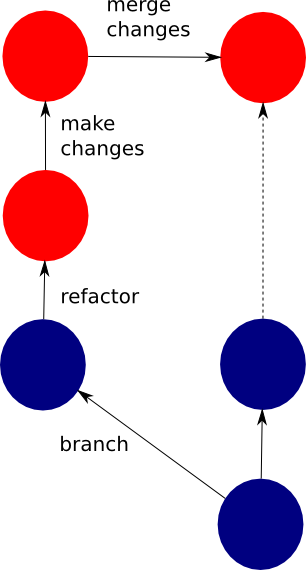
\includegraphics[scale=0.5]{refactorCheckIn}
\end{center}
\caption{Merging changes with refactored code also merges any refactoring}
\end{figure}

The difficulty lies in the fact that not only the functionality that you have added is checked in but also the changes brought about by refactoring.  These refactored changes have not changed how the program functions but have simplified and tidied the code to make the addition of your changes easier. There are some occasions where you may want to make a refactoring available to everyone.  By checking in your refactoring code however, you are forcing others to comply with your vision about how the code should be structured.  This occurs even though you could have no awareness about what changes to the code others have made or intend to make.  Everyone who attempts to check in their code after you will need to merge into a restructured code source that they are unfamiliar with.  This is a recipe for merge based bugs and time wasted doing unnecessary merging.

% Kerievsky also relates a tale about how the lack of knowledge of patterns
% making a particular refactoring look a lot more complex
% \cite{Kerievsky2004}. The different perspectives meant that the programmer
% he refers to as John has a differing opinion that the refactored code was
% not an improvement. This shows that it is not just different functionality
% that influences the need to refactor but sometime the knowledge and
% experience of the developers themselves. It is often the case that two
% developers could have different views about what is an appropriate
% refactoring. This could be because each person brings different skills,
% notices different issues and has a preferred way of visualizing a problem
% and solution.
% 

% 
% then created a branch
% If they attempt to check-in their changes there is the possibility a
% conflict with any of your changes.
% 
% You also need to refactor the code to do your work but both of the
% refactorings are different because they clarify or highlight different
% aspects of the source code.
% 
% If there is some refactoring before any changes are made when the code is
% re-merged with the original project (often called the trunk project) both
% the changes and the refactored code are checked in.




When there is a large change on a separate branch it could be the case that there are multiple check-ins to keep other parts up to date and ensure that there is not too much divergence.  Currently if you have a project where there are periodic check-ins for each development milestone there will be a large impact each time there is a commit. This is because the refactoring for the large refactored project is imposed upon the repository each time it is checked in.

% find an example of a workplace situation where refactoring interferes with
% others


One of these changes which is not catered for by current version control systems is the change of order.  The first person to check-in their code will have no issue as the version control system assumes that all the changes are simply a new revision.  When the second person attempts to reconcile their view there is the possibility of having unnecessary conflicts.  A lot of these conflicts will be with refactored code which although works the same has a different structure.

\subsection{How we would like to address the problem}
We want to be able to maintain views or separate branches that can have different but equivalent refactoring.  When these branches are merged we want to make sure that the equivalent refactored code is not migrated to the view we are merging into.
This is so that people working on the same project can freely refactor with minimal interference to others
When two people refactor the code that they are able to hold their own individual refactoring with minimal change when they are merged.
This also means that there will be less unnecessary merge conflicts when merging code.

We also want to be able to further classify more complex operations in a change set than insert, delete and modify.  When JGit compares files with each other because they are structured it can determine if the file has been moved to a different location in the tree.  At this level JGit can also detect copies and renames.  However once JGit starts comparing source code it loses this structural information.  By giving JGit some idea about the structure in the file it can determine these item at the finer granularity of sections of code rather than at a file basis.

We want to have views that can have different but equivalent refactoring
This is so that people working on the same project can freely refactor with minimal interference to others










\section{What the tool does}
% answer what it does
The refactor categories tool enhances JGit by adding the concept of source code moving to JGits representation of changes.
Currently JGit labels any of the differences it encounters as an insert, a delete, or a modification.  By checking to see if an insert at one point matches a delete at another point it is possible to detect to see if the code block has moved.
To a limited extent the refactor categories tool can also deal with copies and renaming.

By checking to see if an insert at one point matches a delete at another point it is possible to detect to see if the code block has moved.

To a limited extent the refactor categories tool can also deal with copies and renaming.

To a limited extent the refactor categories tool can also deal with copies and renaming.

The refactor categories tool first does a cursory examination of the text differences between two files. It then examines both the differences in executable Java code and the differences between comments and white-space. 
% 
% also checks comments


The refactor categories tool first does a cursory examination of the text differences between two files. It then examines both the differences in executable Java code and the differences in white-space.


\section{How the tool works}
% answer how does stuff

The refactoring difference tool first works out which text has changed using the same method as JGit.
This initial examination returns the differences based on a line by line basis rather than using a smaller granularity.
This means that the set of changes found could still contain code that is comparatively the same.
The set of changes found in using the JGit histogram comparison are then evaluated.
The reason for this is that some items of text could be in a differing order but still be a valid Java program


In order to resolve some limitations with JDime and the text only merge in GIT information about which line numbers are retained after the first text merge.  In JDime these are ignored and the AST is relied upon to hold all the information.  The change set has been taken from the original GIT based diff contains the start and end of the change in both files and what type of change it is (insert delete or modify).  By reusing these line numbers it is possible to figure out which AST items these changes affect. This is done loading the file into the JastAddJ parser to get an AST tree. The line numbers for each item in the tree are then comparing line numbers from the change.

% after finished drill down we have a record of the same changes as JGit
% except now we also have the ASTs

% explain how we limit matching just to the parent of the thing being matched

Comment and white-space are also examined separately as they could give some indication of where code has been moved from or to.

% Comments and white-space cannot be shown in the AST tree so they need to be
% dealt with separately


% insert diagram of how it finds the ASTs that are within the change set
% 
% they are not associated with the AST changes because a comment could be at
% the end of a line and thus associated with the change before.  A multi-line
% comment is normally about the line that follows

\section{Design decisions}
% answer why it does stuff


the tool is based on changes not based on conflicts like JDime is.
the drill down using line numbers

% need to add something about the choice of java and jastaddj

comments
white-space

comparing ASTs
the matcher and how using a score works
finding the best match

% why does it do it for the whole repository

% 
% note: we might want to use some literate programming here11

\section{Limitations of the tool}
The refactor categories tool drills down only on the changes it is harder to investigate any change that has causes side effects in unchanged code.  It is not often that a side effect will be purposely placed in the code as it reflects bad design decisions.  This may however be an issue with bugs.  This also means that the refactor categories tool will not be able to tell when some code is copied but the original remains unchanged. Instead it will assume that it is a completely new insertion of code.
